\documentclass[fleqn,a4paper,12pt]{article}
\usepackage{standalone}		% Zum Einlesen aus anderen .tex-Files
\usepackage{geometry}		% Zur Bearbeitung des Layouts (Ränder,...)
\geometry{left=30mm, right=40mm, bottom=30mm}
\usepackage[german]{babel}
\usepackage[utf8]{inputenc}
\usepackage{amsmath}		% Mathematische Symbole
\usepackage{amssymb}     	% Nochmehr mathematische Symbole
\usepackage{dsfont}      	% Schriftsatz fuer Zahlenmengensymbole
%\usepackage{verbatim}   	% erweiterte Verbatim-Umgebung
\usepackage{alltt}       	% Quasi-Verbatim-Umgebung
\usepackage{fancyhdr}    	% Eigene Kopfzeilen
\usepackage{graphicx}    	% Zum Einbinden von Grafiken
% Einbinden einer eps-Grafik geht so: includegraphics{path}
\usepackage{wrapfig}
\usepackage{lscape}
\usepackage{rotating}
\usepackage{epstopdf}

% Skalierung der Grafiken
\setlength{\unitlength}{1cm}

\pagestyle{fancy}            % Eigene Kopfzeilen verwenden
\frenchspacing               % Kein Extrafreiraum nach Satzzeichen
\setlength{\parindent}{0pt}  % Neue Absaetze nicht einruecken
%\sloppy                     % Schlampige Absatzformatierung
\fussy                       % Penible Absatzformatierung
\linespread{1.5}             % Zeilenabstand

%andere Definitionen
\newcommand{\R}{{\mathbb R}}
\newcommand{\N}{{\mathbb N}}
\newcommand{\Z}{{\mathbb Z}}
\newcommand{\Q}{{\mathbb Q}}
\newcommand{\C}{{\mathbb C}}
\newcommand{\F}{\mathcal{F}}
\newcommand{\less}{\setminus}
\newcommand{\inv}{{}^{-1}}
\newcommand{\Land}{\bigwedge}
\newcommand{\Lor}{\bigvee}

\begin{document}
	  "Ubungsaufgabe 3: \newline
	Messreihe 1000 Würfe mit einem 6-seitigen Würfel: \newline
	5, 4, 2, 4, 5, 6, 3, 2, 5, 3, 4, 2, 1, 1, 5, 1, 1, 2, 1, 6, 4, 6, 1, 4, 5, 3, 2, 3, 2, 1, 1, 2, 6, 2, 5, 2, 5, 6, 4, 6, 4, 5, 2, 2, 3, 1, 2, 5, 5, 4, 5, 5, 4, 5, 2, 2, 5, 4, 3, 5, 5, 4, 2, 4, 3, 1, 5, 4, 1, 6, 5, 4, 5, 4, 2, 1, 4, 1, 2, 6, 1, 1, 5, 3, 5, 3, 1, 6, 4, 6, 1, 6, 2, 5, 4, 4, 2, 6, 1, 3, 4, 2, 2, 5, 3, 3, 2, 5, 6, 2, 3, 3, 3, 6, 3, 1, 4, 2, 1, 5, 6, 6, 3, 2, 3, 3, 5, 6, 3, 1, 4, 5, 6, 3, 1, 1, 4, 3, 1, 2, 3, 6, 3, 2, 3, 4, 2, 4, 6, 4, 3, 4, 3, 2, 4, 5, 5, 4, 3, 3, 2, 4, 4, 5, 5, 6, 4, 2, 6, 6, 5, 5, 6, 6, 2, 3, 1, 2, 3, 2, 5, 1, 3, 3, 2, 4, 5, 2, 4, 5, 3, 6, 5, 3, 5, 5, 2, 6, 4, 3, 6, 5, 5, 2, 1, 5, 5, 2, 1, 3, 2, 5, 3, 2, 2, 6, 3, 5, 4, 3, 1, 1, 5, 6, 5, 6, 3, 2, 3, 1, 6, 6, 3, 5, 3, 2, 5, 3, 2, 5, 2, 5, 3, 5, 2, 2, 1, 5, 4, 3, 6, 6, 2, 6, 3, 2, 3, 2, 4, 5, 4, 6, 3, 1, 3, 1, 3, 4, 1, 1, 1, 6, 2, 1, 5, 4, 5, 6, 2, 4, 1, 4, 2, 6, 3, 6, 1, 2, 2, 2, 3, 5, 3, 6, 2, 5, 2, 6, 5, 1, 2, 2, 5, 4, 2, 5, 6, 3, 1, 3, 1, 3, 6, 5, 3, 5, 2, 6, 4, 3, 4, 2, 2, 6, 6, 1, 2, 1, 4, 5, 1, 3, 3, 1, 6, 5, 4, 2, 1, 5, 4, 6, 6, 1, 2, 4, 1, 4, 3, 2, 2, 1, 3, 4, 3, 6, 2, 1, 4, 3, 6, 2, 1, 2, 5, 2, 6, 1, 2, 3, 1, 4, 3, 5, 6, 1, 6, 5, 2, 4, 4, 4, 2, 1, 3, 3, 3, 3, 1, 3, 6, 6, 2, 4, 1, 2, 5, 2, 6, 1, 6, 3, 2, 1, 5, 4, 3, 4, 3, 1, 6, 2, 4, 1, 5, 2, 5, 3, 4, 6, 3, 2, 6, 3, 4, 6, 1, 5, 2, 5, 5, 5, 6, 5, 2, 5, 1, 4, 2, 3, 2, 5, 5, 6, 1, 1, 2, 4, 6, 3, 4, 5, 4, 4, 1, 4, 4, 1, 2, 6, 6, 6, 1, 4, 3, 3, 5, 6, 5, 2, 3, 4, 4, 6, 5, 1, 4, 3, 3, 1, 4, 4, 4, 4, 6, 6, 1, 4, 4, 1, 1, 3, 3, 4, 4, 4, 4, 4, 1, 3, 3, 4, 3, 3, 3, 5, 6, 1, 1, 1, 2, 6, 3, 1, 5, 5, 1, 5, 5, 3, 3, 5, 6, 2, 6, 2, 3, 1, 4, 6, 4, 2, 2, 5, 5, 2, 6, 5, 5, 5, 1, 4, 4, 4, 4, 5, 5, 5, 6, 6, 4, 6, 1, 2, 6, 6, 2, 5, 1, 6, 1, 3, 1, 1, 2, 3, 1, 1, 1, 1, 1, 2, 4, 6, 3, 4, 6, 6, 3, 4, 5, 4, 4, 2, 3, 2, 4, 1, 2, 3, 5, 3, 6, 3, 6, 4, 4, 6, 3, 5, 4, 1, 4, 5, 3, 3, 5, 4, 2, 6, 4, 4, 1, 4, 1, 1, 4, 4, 6, 3, 6, 3, 2, 4, 6, 1, 3, 6, 6, 6, 3, 1, 5, 6, 6, 3, 6, 6, 5, 1, 3, 6, 1, 6, 2, 5, 4, 6, 1, 5, 5, 3, 4, 4, 6, 4, 1, 2, 6, 5, 6, 3, 6, 2, 1, 1, 2, 3, 4, 5, 4, 3, 6, 5, 6, 5, 4, 4, 1, 6, 6, 2, 1, 6, 1, 5, 2, 3, 6, 4, 1, 5, 5, 2, 2, 2, 3, 3, 4, 6, 2, 4, 2, 1, 2, 6, 1, 3, 3, 1, 6, 4, 1, 4, 6, 3, 2, 1, 4, 2, 2, 1, 1, 1, 2, 4, 5, 1, 5, 5, 4, 5, 6, 3, 1, 5, 1, 1, 5, 4, 2, 2, 2, 5, 3, 6, 6, 3, 5, 4, 4, 1, 2, 4, 5, 6, 4, 5, 1, 6, 2, 2, 2, 5, 5, 2, 3, 6, 5, 6, 6, 2, 2, 1, 1, 5, 6, 4, 3, 2, 2, 3, 2, 5, 1, 1, 2, 5, 1, 4, 6, 2, 1, 2, 2, 4, 4, 1, 6, 2, 6, 3, 5, 3, 1, 3, 5, 2, 4, 6, 3, 5, 5, 2, 1, 3, 3, 5, 3, 4, 5, 1, 2, 2, 2, 6, 6, 1, 2, 6, 1, 1, 3, 2, 3, 2, 1, 6, 2, 6, 5, 6, 3, 1, 5, 3, 2, 6, 5, 6, 4, 3, 1, 1, 1, 3, 4, 2, 3, 4, 1, 5, 4, 3, 1, 5, 6, 4, 3, 6, 5, 2, 1, 2, 5, 2, 1, 2, 2, 2, 2, 5, 4, 2, 2, 3, 3, 5, 4, 3, 2, 3, 1, 4, 4, 6, 3, 5, 1, 1, 2, 6, 3, 2, 4, 5, 1, 5, 4, 5, 5, 4, 1, 1, 5, 6, 6, 5, 6, 5, 5, 2, 5, 1, 1, 1, 2, 5, 5, 5, 1, 5, 6, 2, 4, 5, 5, 6, 6, 6, 3, 2, 2, 4, 2, 5, 5, 4, 4, 5, 4, 2, 5, 1, 1, 6, 1, 4, 6, 6, 1, 4, 6, 2, 4, 5, 6, 3, 6, 3, 4, 2, 4, 4, 2, 6, 5, 5, 1, 2, 5, 6, 1, 5, 3, 2, 5, 3, 6, 2, 2, 4, 1, 4, 4, 5, 4, 3, 1, 6 \newline
	\textbf{Häufigkeiten:}
	\begin{center}
		\begin{tabular}{ | l | l | l | }
			\hline
			Augenzahl & Anzahl der Würfe & relative Häufigkeit \\ \hline
			1 & 164 & 0.164 \\ \hline
			2 & 177 & 0.177 \\ \hline
			3 & 158 & 0.158 \\ \hline
			4 & 164 & 0.164 \\ \hline
			5 & 175 & 0.175 \\ \hline
			6 & 162 & 0.162 \\ \hline
		\end{tabular}  
	\end{center}
	\textbf{Berechnung des Medians:} \newline
	$0.164 + 0.177 + 0.158 = 0.499 \leq 0.5$ \newline
	$0.164 + 0.177 + 0.158 + 0.164 = 0.663 > 0.5$ \newline
	Der Median ist also 3 (der dritte Summand stellt Augenzahl 3 da). \newline
	\textbf{Modalwert:} \newline
	$0.177 > 0.175 > 0.164 > 0.162 > 0.158$ \newline
	Der Modalwert ist also 2. \newline
	\textbf{Mittwelwert:} \newline 
	$m_1 = \sum_{i=0}^{n-1} x_i p_i$ \newline
	$m_1 = 1*0.164 + 2*0.177 + 3*0.158 + 4*0.164 + 5*0.175 + 6*0.162 \approx 3.5$ \newline
	\textbf{Standardabweichung:} \newline
	$s = \sqrt{\sum_{i=0}^{n-1} (x_i-m_1)^2 p_i}$ \newline
	$s = \sqrt{(1-3.495)^2*0.164 + (2-3.495)^2*0.177 + (3-3.495)^2*0.158} \\\overline{+ (4-3.495)^2*0.164 + (5-3.495)^2*0.175 + (6-3.495)^2*0.162} \approx 1.7$ \newpage
	\begin{figure}
		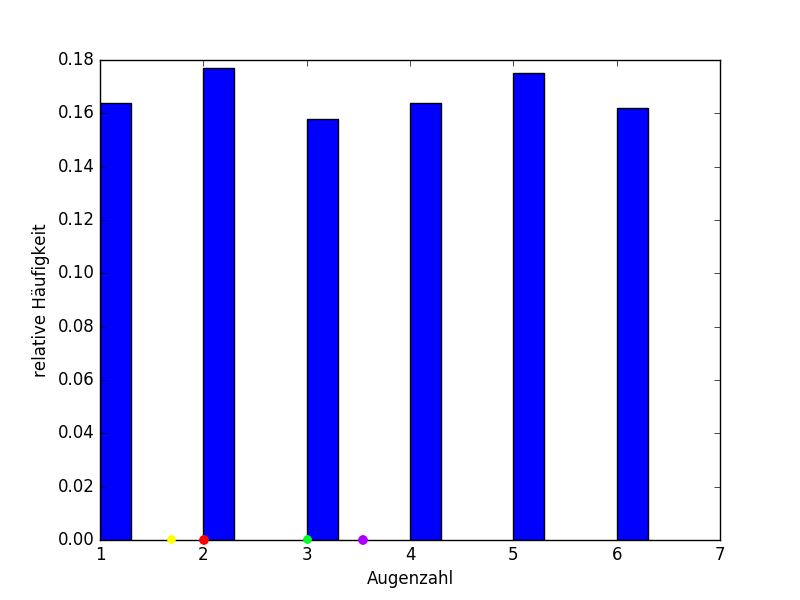
\includegraphics[width=1.0\textwidth]{A03_histo.png}
		\caption{Histogramm für 1000 Würfe mit einem 6-seitigen Würfel. \newline gelb: Standardabweichung, rot: Modalwert, grün: Median, violett: Mittwelwert}
	\end{figure}
	\textbf{Entropie:} \newline
	$H = \sum_{i=0}^{n-1} p_i log_2(\frac{1}{p_i})$ \newline
	$H = 0.164*log_2(\frac{1}{0.164}) + 0.177*log_2(\frac{1}{0.177}) + 0.158*log_2(\frac{1}{0.158}) + 0.164*log_2(\frac{1}{0.164}) + 0.175*log_2(\frac{1}{0.175}) + 0.162*log_2(\frac{1}{0.162}) \approx 2.58373$ \newline
	\textbf{Max. Entropie:} \newline
	$H_{max} = log_2(n)$ \newline
	$H_{max} = log_2(6) \approx 2.58496$ \newline
	\textbf{Redundanz:} \newline
	$R = H_{max} - H = 2.58496 - 2.58373 \approx 0.001$ \newline
	Die Redundanz ist sehr klein.
\end{document}